% **
% Revisão da literatura.
% *

\section{PANORAMA HISTÓRICO DA CRIPTOGRAFIA}

A criptografia é uma ferramenta indispensável para a proteção de informações.
Derivada do grego "kriptos", que significa "secreto", e "graphia", que se
refere à "escrita", é uma ferramenta indispensável para a proteção de
informações (Pabón Cadavid, 2010, p. 59) ou (Filho e Azeredo, 2017, p. 23).
Envolve a utilização de algoritmos para transformar a informação original em um
formato indetectável e inacessível a indivíduos sem autorização. Ela desempenha
um papel crucial na garantia da segurança da transmissão de informações,
especialmente em redes ou ambientes considerados inseguros (Viana \textit{et
	al}, 2022, p. 226).

Com sua origem na antiguidade, a criptografia já era utilizada em situações
militares complexas, conforme relatados Heródoto; destacou-se ainda mais
sobre figuras históricas como Júlio César, que utilizou técnicas
esteganográficas e criptográficas em suas comunicações para garantir a
confidencialidade das informações. A introdução dos sistemas elétricos de
transmissão de informações impulsionou a criptografia para uma
nova trajetória, tornando-se o precursora do que conhecemos hoje (Pabón
Cadavid, 2010, p. 61-63).

\subsection{Origem e desenvolvimento da criptografia}

A era moderna, especialmente após a Segunda Guerra Mundial, trouxe avanços
tecnológicos notáveis na criptografia. Durante esse período, houve uma expansão
significativa na pesquisa e desenvolvimento em criptografia, o que despertou
não apenas o interesse das forças armadas e dos governos, mas também do público
em geral. Com o crescimento da pesquisa e do desenvolvimento no campo, houve a
criação de sistemas computacionais avançados para fins de criptografia,
destacando-se como ferramentas essenciais para a segurança da informação (Pabón
Cadavid, 2010, p. 64).

Neste cenário, grandes descobertas, como a máquina de Charles Babbage e as
bombas de Turing de Alan Turing, desempenharam um papel crucial. Essas
invenções, originalmente voltadas para o desciframento de códigos, se tornaram
fundamentais para o desenvolvimento da tecnologia informática atual. É
importante ressaltar que sem esses desenvolvimentos pioneiros na criptografia,
a revolução da tecnologia da informação poderia ter tomado um curso bastante
diferente, evidenciando o papel crucial da criptografia na evolução da
tecnologia (Pabón Cadavid, 2010, p. 64).

A criptografia moderna, embora mantenha a essência de sua prática histórica, se
tornou amplamente complexa devido ao avanço tecnológico. Sua execução não se
limita mais à simples reorganização do alfabeto, mas incorpora algoritmos
matemáticos complicados para cifrar mensagens. Da mesma forma, a tarefa de
"quebrar" códigos criptográficos, a criptoanálise, sai da capacidade humana de
observar padrões de repetição de letras, tornando-se dependente da potência de
supercomputadores. Dessa forma, se torna quase impossível criar códigos seguros
e descriptografá-los sem um sólido conhecimento em matemática, considerável
poder de processamento de dados e um substancial investimento financeiro
(Abreu, 2017, p. 28)

\subsection{Adaptação da criptografia ao mundo moderno}

No mundo contemporâneo, cada vez mais imerso em digitalização e conectividade,
não podemos ignorar a preponderância e a importância vital da criptografia. Há
uma presença profunda e abrangente da tecnologia em nossas vidas cotidianas,
desde comunicação pessoal, transações financeiras até a infraestrutura crucial
de qualquer nação. Tudo isso cria um cenário onde a segurança dos dados online
se torna não apenas desejável, mas uma absoluta necessidade.

Nesse cenário, a criptografia emerge como um componente soberano na garantia da
segurança e privacidade do usuário na internet. Este foco elevado na
criptografia é compreensível considerando que ela proporciona um canal seguro
para troca de informações delicadas nesse mar aberto e incerto que é a web
(Viana \textit{et al}, 2022, p. 231-236). A criptografia não apenas permeia o
tecido de nossas interações online como indivíduos, mas também desempenha um
papel crucial para entidades empresariais e governamentais. Seu alcance não se
restringe somente a aplicativos e websites; na verdade, ela é de vital
importância para sistemas mais complexos e intrincados.

É nesses sistemas que evidenciamos sua relevância no setor privado. As trocas de
informações confidenciais são recorrentes nas interações empresariais, e a
criptografia se torna um escudo protetor, guardião da integridade dessas
informações. Além disso, situações de hostilidade, como períodos de guerra ou
conflito, reforçam ainda mais a necessidade de mensagens codificadas para garantir
a segurança e evitar deturpações (Andria; Gondim; Salomão, 2019, p. 31-36).
Por outro lado, as transações financeiras se tornaram primariamente digitais devido
ao conveniente avanço tecnológico. Essa transição para o meio digital das
transações financeiras, junto com atividades comerciais e assuntos corporativos
sensíveis, certamente exigem um nível de confidencialidade que somente a criptografia
pode providenciar adequadamente.

Cada dia mais pessoas estão se deliciando com a comodidade que a internet
proporciona, sem se dar conta de que cada transação, cada troca de dados
seguros, é facilitada e resguardada por diversos sistemas de criptografia que
trabalham incansavelmente em segundo plano. Por esse motivo, podemos afirmar
sem hesitação que a criptografia não é apenas um luxo, mas uma necessidade
crucial que proporciona a segurança e confiança tão necessárias na atual era
digital (Andria; Gondim; Salomão, 2019, p. 31-36). Com tudo isso em mente,
fica claro que sem a presença vital da criptografia, o ciberespaço atual seria
um lugar muito mais perigoso e imprevisível de se navegar.

\subsection{Os impasses legais na utilização da criptografia}

Na era da economia digital avançada e da transformação digital disseminada na
vida cotidiana, a demanda por sistemas seguros e confiáveis está em progressivo
crescimento. Ao atender essas demandas, a criptografia emerge como uma
protagonista estratégica. Ela atua como uma poderosa ferramenta na salvaguarda
de dados, assegurando que as informações transmitidas permaneçam inacessíveis a
olhares indesejados (Viana \textit{et al}, 2022, p. 231-232). No entanto,
lançamos nosso olhar a um peculiar dilema quando o 'olhar indesejado' que tenta
acessar essas informações se identifica como o próprio Estado.

A capacidade da criptografia em manter os dados impenetráveis e invioláveis
frequentemente se torna o núcleo dos debates legais entre as grandes empresas
tecnológicas e os governos. Estas discussões centram-se na dificuldade ou, em
muitos casos, na impossibilidade de se violar a privacidade que esses sistemas
criptográficos garantem. Podemos observar esse conflito através de casos
emblemáticos, como o do aplicativo de mensagens instantâneas WhatsApp,
bloqueado três vezes no Brasil por se recusar a fornecer o conteúdo de
comunicações dos investigados em processos criminais (Abreu, 2017, p. 28).

Seguindo essa mesma linha, podemos revisitar o conflito de 2015 entre a Apple e
o governo dos EUA. A face a face de discordâncias aconteceu por causa dos
robustos mecanismos de criptografia utilizados nos iPhone, considerados
invioláveis pelo governo. Este evento sublinha a tensão inerente na relação
entre os Estados e a criptografia: é uma ferramenta que uso, mas rejeito seu
uso por outros, especialmente quando esses "outros" são considerados potenciais
adversários (Abreu, 2017, p. 28). Essa dualidade mostra a complexidade da
relação entre segurança, privacidade e governança na era digital.

\subsection{Criptografia: um olhar para o futuro}

Portanto, a importância da criptografia não é uma questão só do passado ou do
presente. Sua relevância se perpetua ao longo do tempo, evoluindo constante e
adaptativamente para atender necessidades emergentes de segurança e para
sustentar a confiabilidade na digitalização crescente (Viana \textit{et al},
2022, p. 234). A habilidade de cifrar mensagens, permitindo uma comunicação
segura e privada, volta-se cada vez mais indispensável em uma sociedade que é,
ao mesmo tempo, altamente digital e globalmente interconectada.

A criptografia, cujo papel tem sido de relevância para a humanidade desde os
tempos antigos, certamente continuará a ser uma peça chave no nosso futuro
digital. Por garantir a privacidade e a segurança das informações, a
criptografia é uma ferramenta crucial para proteger dados em um mundo que se
torna cada dia mais dependente da tecnologia e da digitalização. Sua
relevância, longe de diminuir, só tem a crescer e se adaptar para atender às
novas demandas e necessidades de segurança que irão surgir.

\section{FUNDAMENTOS E CARACTERÍSTICAS DA CRIPTOGRAFIA}

\subsection{Entendendo a criptografia simétrica}

\begin{figure}[h!] \centering
	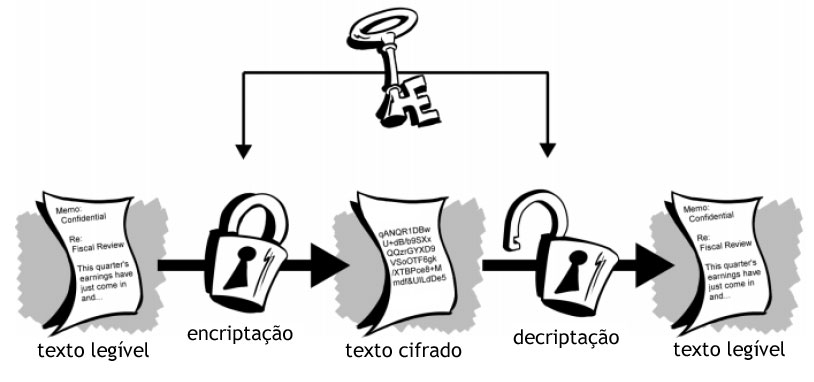
\includegraphics[width=0.7\textwidth]{Imagens/ilustracao_do_processo_de_criptografia_simetrico}
	\caption{Ilustração do processo de criptografia Simétrico}
	Fonte: Seragiotto, 2023, p. ?
\end{figure}

A criptografia simétrica, de processo ilustrado na Figura 1, é um dos
principais métodos de criptografia, onde é usada uma única chave tanto para
criptografar quanto para descriptografar os dados. Este sistema é eficiente e
rápido, onde o remetente utiliza a chave para transformar a mensagem em um
formato ilegível, sendo então revertida no lado do destinatário usando a mesma
chave (Viana \textit{et al}, 2022, p. 235-236)

\begin{CitacaoLonga}
	Essencialmente, quando a origem (ALFA) cifra uma mensagem, ele utiliza um
	algoritmo de ciframento para transformar o conteúdo em claro da mensagem em
	texto cifrado. Quando o destino (BRAVO) decifra uma mensagem, ele utiliza o
	algoritmo de deciframento correspondente para converter o texto cifrado de novo
	em uma mensagem clara. Se um intruso (CHARLIE) conhecer o algoritmo de
	ciframento, ele poderia decifrar uma mensagem cifrada tão facilmente quanto o
	destino (BRAVO). A solução no uso da criptografia de chave privada propõe que
	quando a origem (ALFA) cifra uma mensagem, ele utilize um algoritmo de
	ciframento e uma chave secreta para transformar uma mensagem clara em um texto
	cifrado. O destino (BRAVO), por sua vez, ao decifrar a mensagem, utiliza o
	algoritmo de deciframento correspondente e a mesma chave para transformar o
	texto cifrado em uma mensagem em claro. O intruso (CHARLIE), por não possuir a
	chave secreta, mesmo conhecendo o algoritmo, não conseguirá decifrar a
	mensagem. A segurança do sistema passa a residir não mais no algoritmo e sim na
	chave empregada. É ela (chave privada) que agora, no lugar do algoritmo, deverá
	ser mantida em segredo pela origem (ALFA) e destino (BRAVO) (Oliveira, 2012, p. 3)
\end{CitacaoLonga}

Entretanto, um desafio crítico ao utilizar esse sistema é o compartilhamento
seguro da chave que deve ser efetuado entre o remetente e o destinatário. Este
processo precisa ser seguro para evitar que indivíduos mal-intencionados
interceptem a chave e tenham acesso à informação enviada (Viana \textit{et al},
2022, p. 236)

\subsection{Entendendo a criptografia assimétrica}

\begin{figure}[h!] \centering
	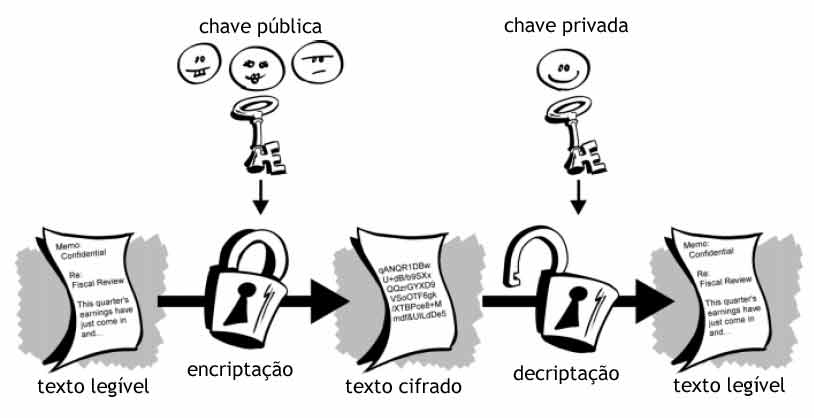
\includegraphics[width=0.7\textwidth]{Imagens/ilustracao_do_processo_de_criptografia_assimetrico}
	\caption{Ilustração do processo de criptografia Assimétrico}
	Fonte: Seragiotto, 2023, p. ?
\end{figure}

Contrastando com a criptografia simétrica, temos a criptografia assimétrica, de
processo ilustrado na Figura 2, também conhecida como criptografia de chave
pública. Aqui, um par de chaves é usado, sendo elas a chave pública, que pode
ser compartilhada abertamente, e uma chave privada, que deve ser mantida em
sigilo somente pelo destinatário da mensagem (Viana \textit{et al}, 2022, p.
238)

\begin{CitacaoLonga}
	Essencialmente, o destino (BRAVO) e todos os que desejam comunicar-se de modo
	seguro geram uma chave de ciframento e sua correspondente chave de
	deciframento. Ele mantém secreta a chave de deciframento, esta é chamada de sua
	chave privada. Ele torna pública a chave de ciframento, esta é chamada de sua
	chave pública. A chave pública realmente condiz com seu nome. Qualquer pessoa
	pode obter uma cópia dela. O destino (BRAVO) inclusive encoraja isto,
	enviando-a para seus amigos ou publicando-a na internet. Assim, O intruso
	(CHARLIE) não tem nenhuma dificuldade em obtê-la. Quando a origem (ALFA) deseja
	enviar uma mensagem ao destino (BRAVO), precisa primeiro encontrar a chave
	pública dele. Feito isto, ela cifra sua mensagem utilizando a chave pública do
	destino (BRAVO), despachando-a em seguida. Quando o destino (BRAVO) recebe a
	mensagem, ele a decifra facilmente com sua chave privada. O intruso (CHARLIE),
	que interceptou a mensagem em trânsito, não conhece a chave privada do destino
	(BRAVO), embora conheça sua chave pública. Mas este conhecimento não o ajuda a
	decifrar a mensagem. Mesmo a origem (ALFA), que foi quem cifrou a mensagem com
	a chave pública do destino (BRAVO), não pode decifrá-la agora. (Oliveira, 2012,
	p. 4)
\end{CitacaoLonga}

Para enviar uma mensagem utilizando criptografia assimétrica, a chave pública
do destinatário é usada pelo remetente para criptografar a mensagem. Esta só
pode ser decriptada e lida pelo destinatário que possui a chave privada
correspondente. Isso adiciona uma camada extra de segurança à mensagem, pois a
chave privada é exclusiva do destinatário (Viana \textit{et al}, 2022, p. 240)

\subsection{Contrapontos entre criptografia simétrica e assimétrica}

A criptografia simétrica e a criptografia assimétrica possuem diferenças
essenciais que ditam suas aplicações ideais. A criptografia simétrica é rápida
e eficiente, tornando-a ideal para a codificação de conteúdos de mensagens.
Isso garante a confidencialidade de dados no processo de transmissão. No
entanto, as abordagens simétricas encontram suas principais desvantagens na
complexidade do gerenciamento e distribuição de chaves (Oliveira, 2012, p. 8).

Gerenciar e distribuir chaves é um desafio na criptografia simétrica, pois
exige um canal seguro para o compartilhamento das chaves entre emissor e
receptor. Esse processo se torna complicado, especialmente quando há um grande
número de participantes na transmissão de dados. Isso torna a gerência das
chaves extremamente difícil e vulnerável a falhas (Oliveira, 2012, p. 8).

Em contrapartida, a criptografia assimétrica resolve os problemas de
gerenciamento e distribuição de chaves que são inerentes à criptografia
simétrica. Embora seja mais lenta devido ao seu alto grau de complexidade, ela
fornece um nível maior de segurança. Isso ocorre através da separação das
chaves em públicas e privadas (Oliveira, 2012, p. 8).

Na criptografia assimétrica, a chave pública pode ser distribuída livremente.
Enquanto isso, a chave privada, utilizada para decodificar o documento
codificado, é conhecida apenas pelo seu proprietário. Além disso, este tipo de
criptografia é ideal para a distribuição de chaves e para assinatura digital.
Isso garante não apenas a confidencialidade, mas também a autenticidade e a
integridade das mensagens (Oliveira, 2012, p. 8).

% \begin{table}[h!]\centering
% 	\caption{Quadro comparativo}
% 	\begin{tabular}{ p{7.3cm} |  p{7.3cm}}
% 		\hline
% 		\textbf{Criptografia simétrica ou chave privada} & \textbf{Criptografia assimétrica ou chave pública} \\
% 		\hline
% 		Rápida                                           & Lenta                                              \\
% 		\hline
% 		Gerência e distribuição das chaves é complexa    & Gerência e distribuição das chaves é simples       \\
% 		\hline
% 		Não oferece assinatura digital                   & Oferece assinatura digital                         \\
% 		\hline
% 	\end{tabular}
% 	%
% 	\vspace*{0.4cm}\\ % Não apagar esta linha
% 	Fonte:  Oliveira, 2012,  p. 8
% \end{table}

% A Tabela 1 sumariza as características principais de cada abordagem da
% criptografia. Nota-se que a criptografia simétrica, apesar de ser mais rápida,
% é mais complexa em relação à gerência e distribuição de chaves e não oferece a
% funcionalidade de assinatura digital. Por contrapartida, a criptografia
% assimétrica, ainda que seja mais lenta, apresenta simplicidade no manejo e
% distribuição de chaves e proporciona a ferramenta de assinatura digital.

Ambas os sistemas de criptografia possuem suas vantagens e desvantagens.
Enquanto a criptografia simétrica é rápida e eficiente, a segurança do
compartilhamento de chaves é um desafio. Por outro lado, a criptografia
assimétrica fornece uma segurança extra com a separação de chaves em pública e
privada, mas pode ser mais lenta devido ao seu maior nível de complexidade. A
escolha do tipo de criptografia a ser usado depende das necessidades
específicas de segurança de cada situação.
